\subsection{Designer Personas} \label{p6section:results}

%We  trained  3  models  for  each  representation  and  problem configuration. To analyze these models, we collected 40 generated levels for each model.  To generate the levels, 40 different random level layouts were generated, the models were then tasked with modifying these random layouts into good levels.   We  analyzed  the  final  modified  levels  using  different change percentages, ranging from0%to100%, where thepercentage represents the fraction of tiles the agent is allowedto change during inference

%To understand the typical progress of designers and validate the clustering, we visualize how typical design sessions traverse the various clusters. These trajectories  are  then  clustered  to  find  a  small  handful of designer personas.

\begin{figure*}[t]
    \centering
     \subfloat[\textsc{Architectural-focus}\label{p6subfig-1:dummy}]{%
       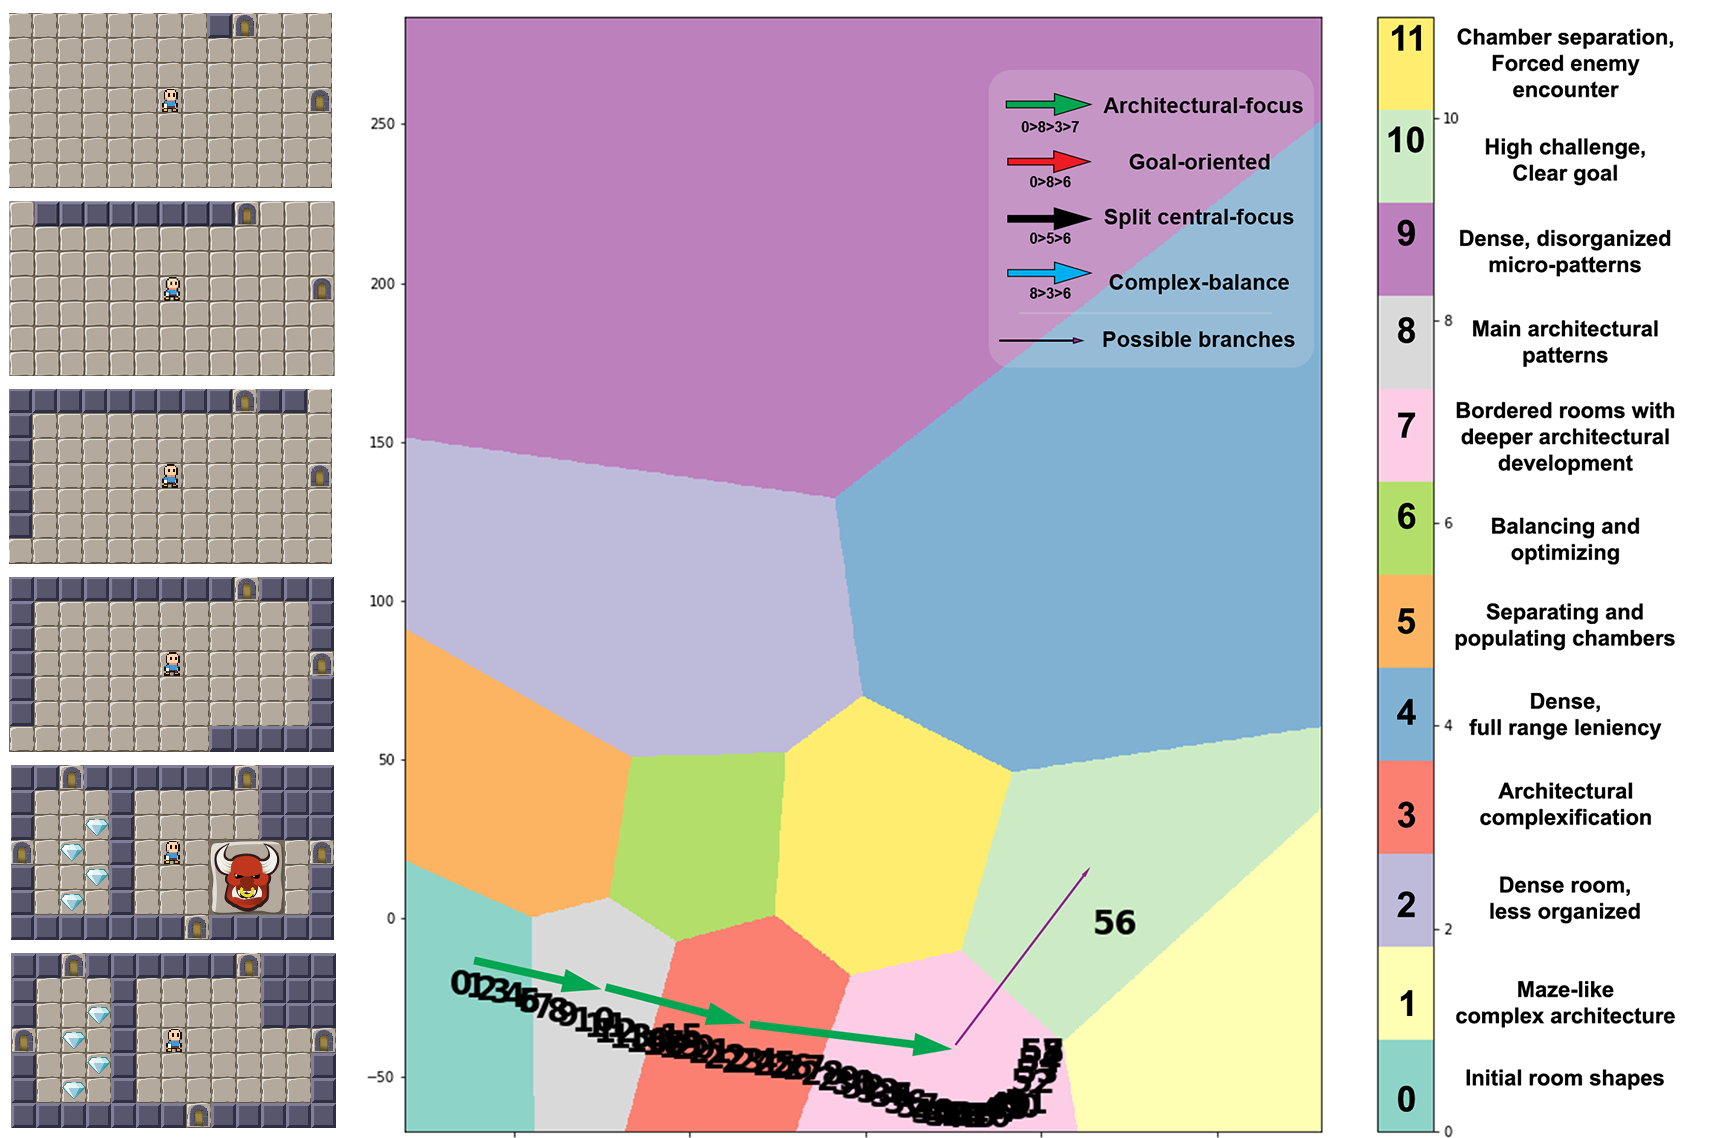
\includegraphics[width=0.45\textwidth]{figures/1.png}
     }
     \hfill
     \subfloat[\textsc{Goal-oriented}\label{p6subfig-2:dummy}]{%
       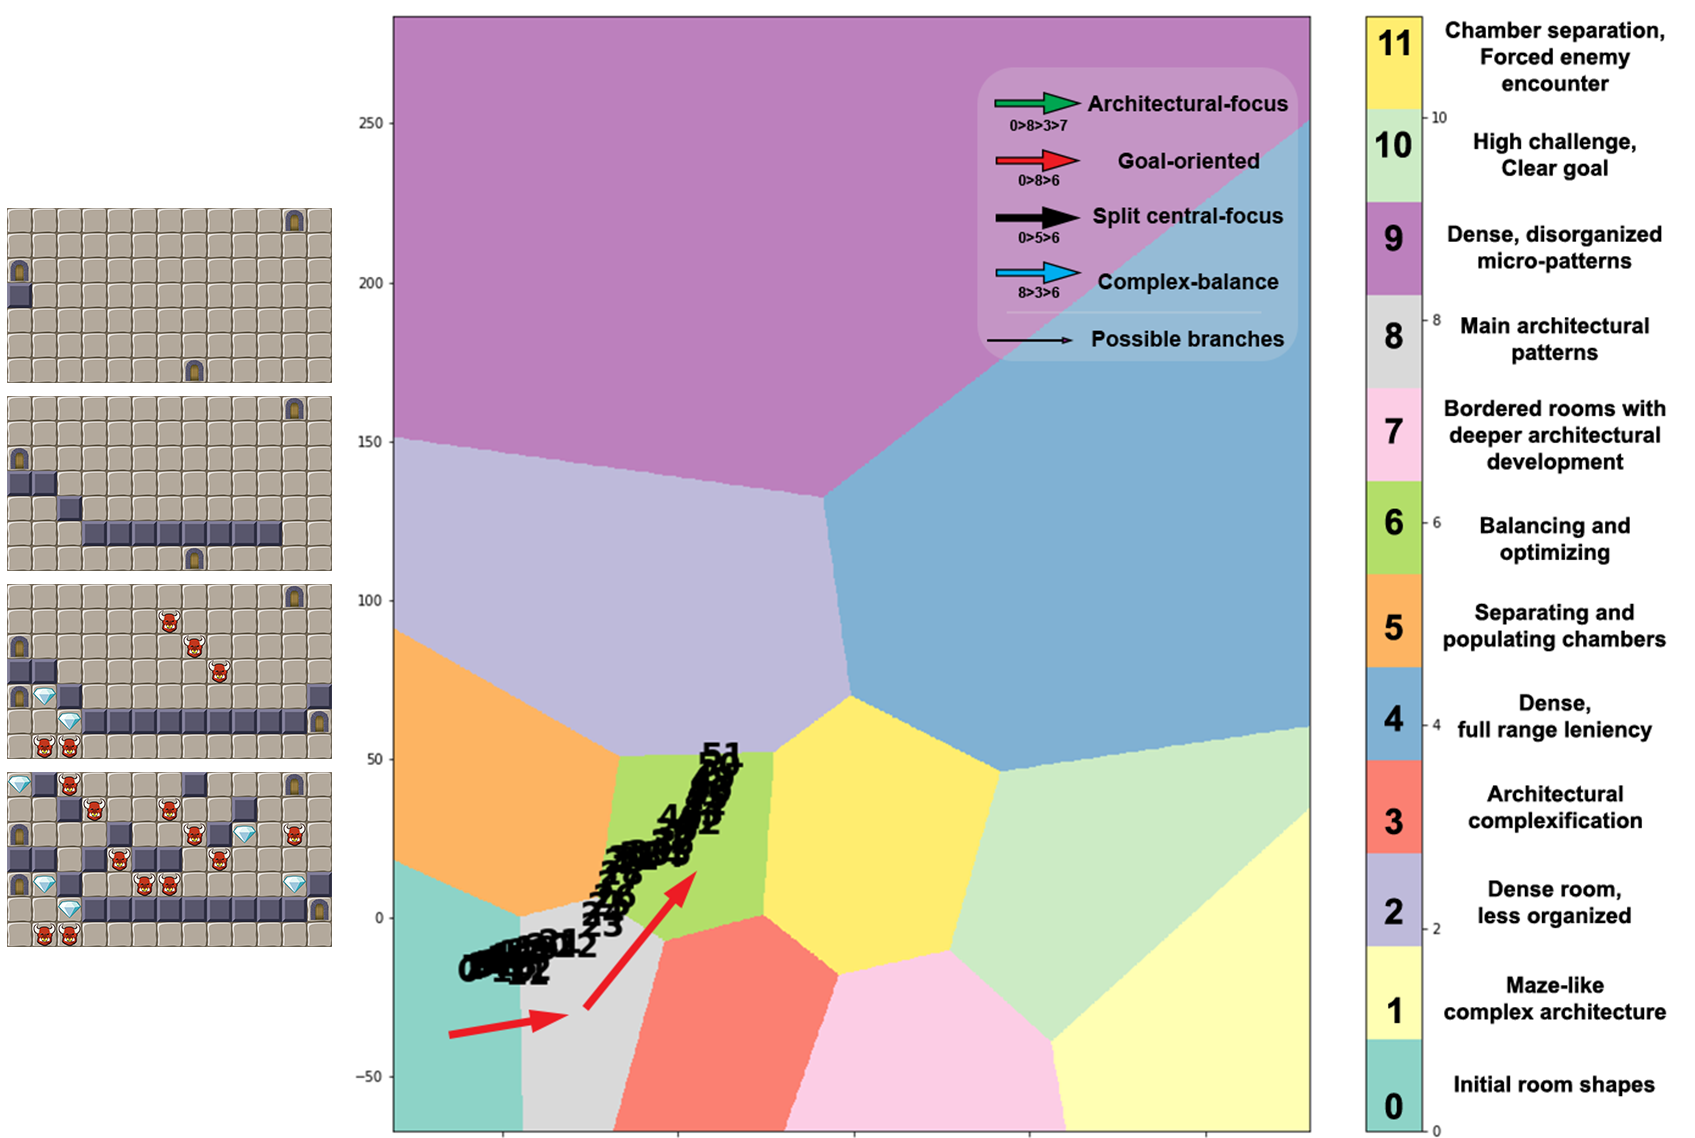
\includegraphics[width=0.45\textwidth]{figures/2.png}
     }\hfill
    %  \medskip
     \subfloat[\textsc{Split central-focus}\label{p6subfig-3:dummy}]{%
       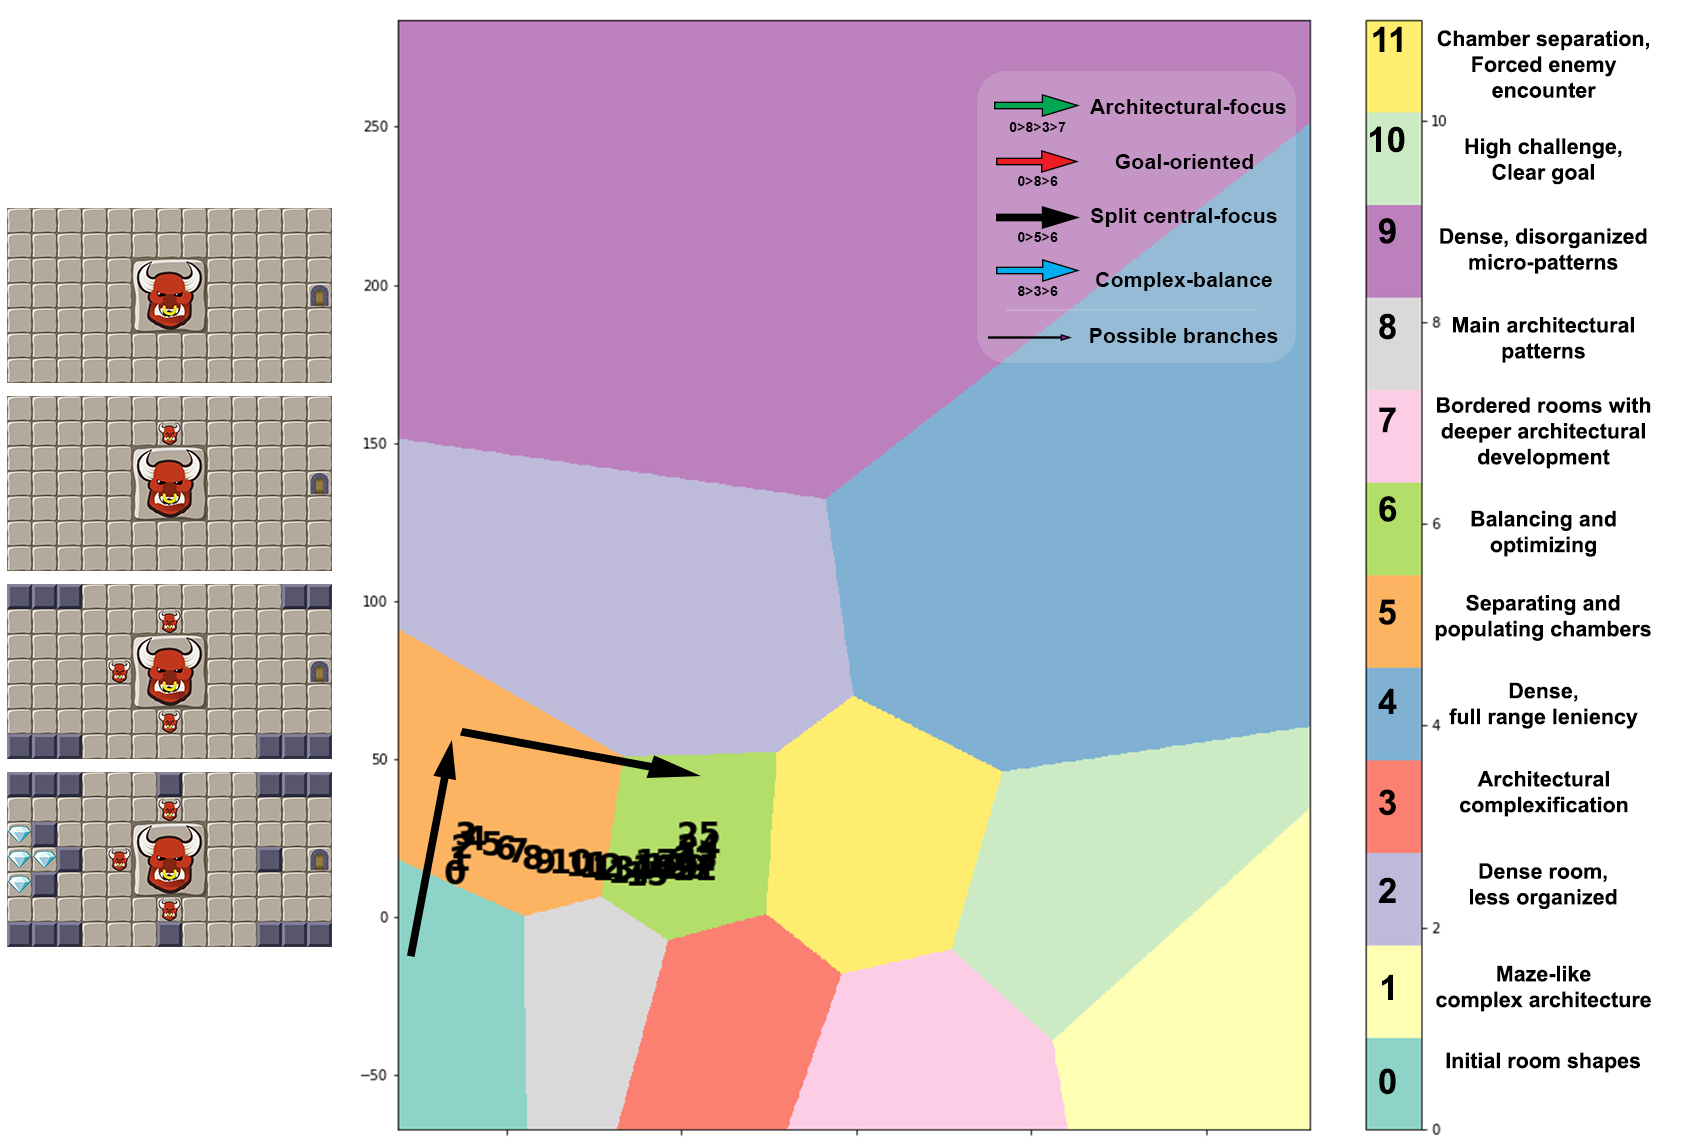
\includegraphics[width=0.45\textwidth]{figures/3.png}
     }
     \hfill
     \subfloat[\textsc{Complex-balance}\label{p6subfig-4:dummy}]{%
       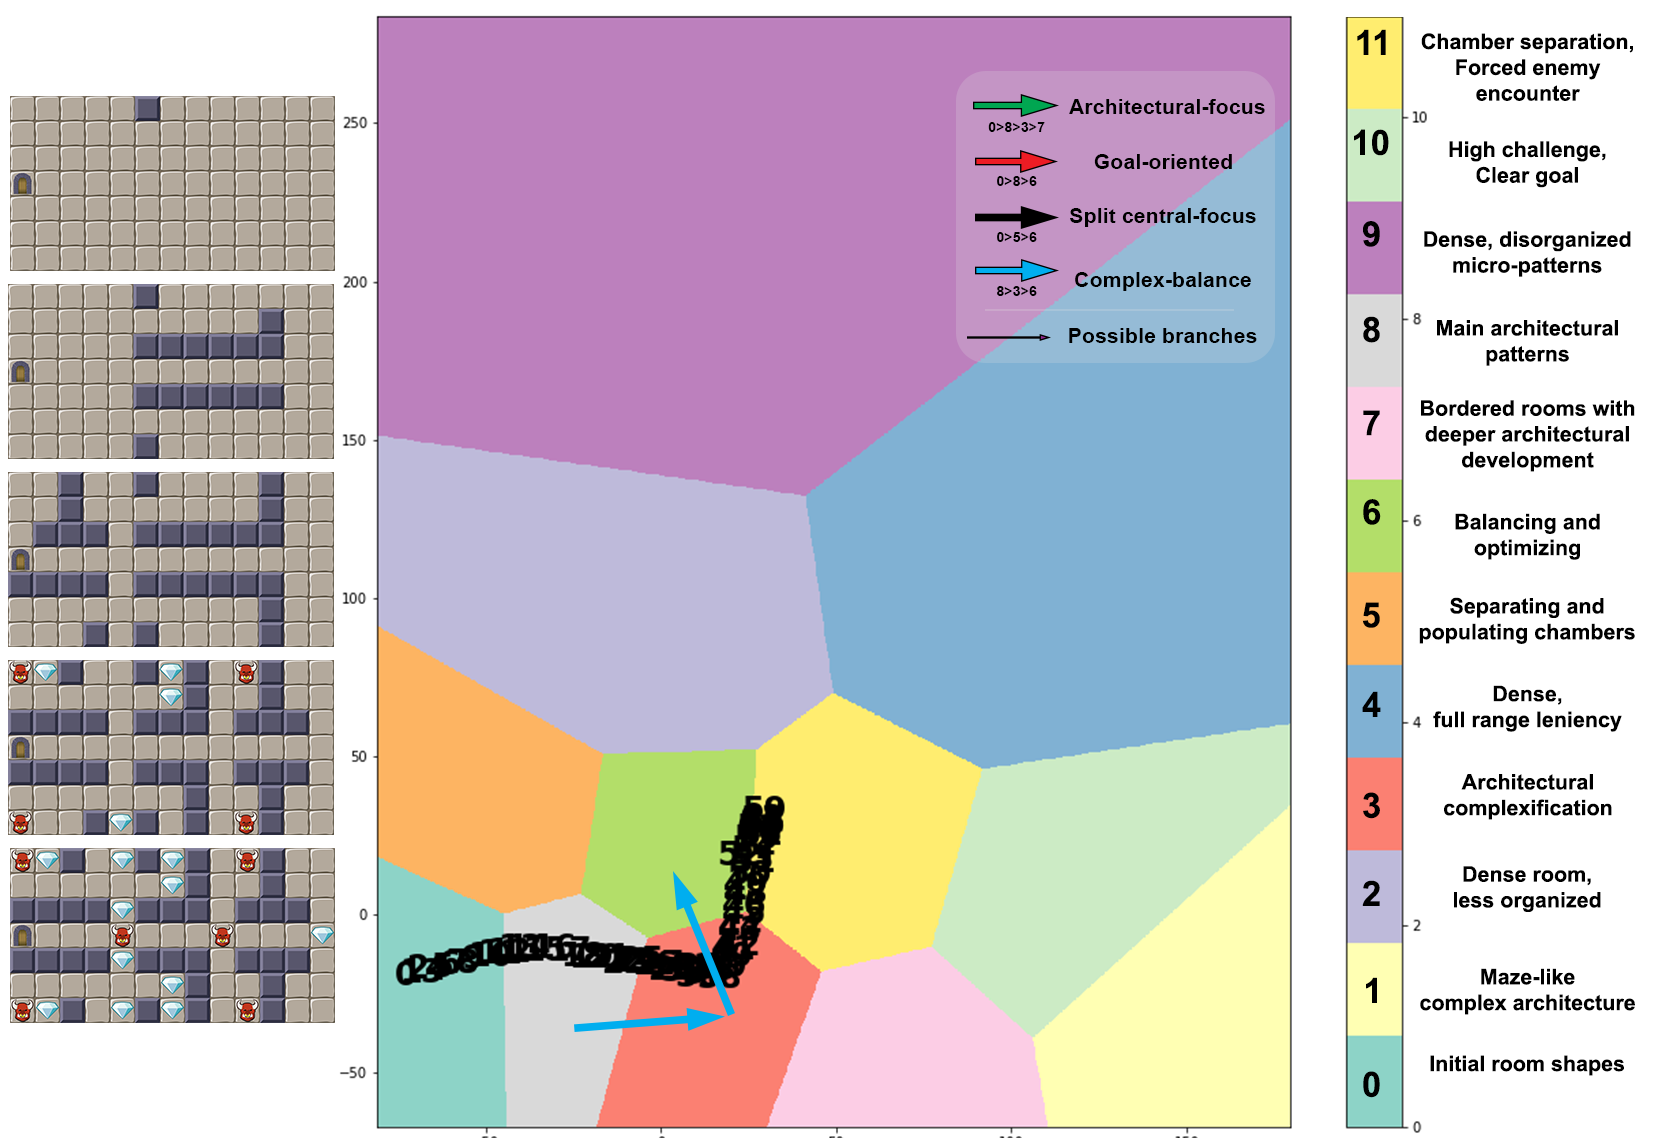
\includegraphics[width=0.45\textwidth]{figures/4.png}
     }
    
    \caption{Examples of each of the archetypical paths from one of the frequent sequences used to create the clusters. To the left of each subfigure, we present each key step in the trajectory i.e. when the design entered a new cluster. (a) presents the \textsc{Architectural-focus} archetypical path where the focus is firstly on creating the structural design of the rooms; the design process jumps back and forth suddenly to cluster 10 (one of the possible branches) due to the designer adding a boss, and removing it immediately. (b) presents the \textsc{Goal-oriented} archetypical path where the design focus on a minimal structure complexity and mix between adding structural changes and enemies/treasures. (c) shows the \textsc{Split central-focus} archetypical path where, intentionally, the designer creates a center obstacle with a boss and build around it. Finally, (d) presents the \textsc{Complex-balance} archetypical path; the design focuses on building complex, uncommon structures first and then add some goal to it with enemies and treasures, taking advantage of the spaces.}
    \label{p6fig:archetypical-examples}
\end{figure*}


Once we created, evaluated, and labeled the clusters, we were able to cluster and visualize the paths of a typical design session. Figure \ref{p6fig:paths-designers} presents an example of the design sessions, where we cluster each step of the design. This sequential process revealed that there is an interesting continuity between clusters, even capturing when a designer probably applied one of the procedural suggestions due to bigger steps in the design style clusters. Further, through this process, we could understand the progress of designers in their design process and represent their trajectory in relation to the traversed clusters rather than individual editions.

\subsubsection{Unique Trajectories}

Using the clusters in Figure \ref{p6fig:all-clusters}, we clustered the design session of all the $180$ designs and collected the unique trajectories that arose from traversing the various clusters. These unique trajectories varied in the starting point, length, and end-point, however, when analyzing the trajectories we identified common patterns among them. They had a similar shape as the following $Unique=$\{0\textgreater8\textgreater4\textgreater7\textgreater10\}, where the first and last element of the sequence are respectively, the starting- and end-points, with all the unique intermediate steps in between.

To gather the common patterns from the trajectories, we applied the Generalized Sequential Pattern (GSP) algorithm, which locates frequent subsequences in the analyzed trajectories. For instance, given three trajectories (a) \{5\textgreater1\textgreater3\textgreater11\textgreater9\}, (b) \{5\textgreater1\textgreater3\textgreater11\textgreater4\, and (c) \{0\textgreater1\textgreater3\textgreater11\}, none of these is a perfect match in its entirety, but GSP can spot that subsequences \{1\textgreater3\textgreater11\}, \{1\textgreater3\}, \{3\textgreater11\}, among others, appear with frequency $= 3$.

%(2) obtain only 1 pattern ($\{5>1>3>11\}$) with frequency=2, if searching from starting points. Finally, using GSP, we find $\{5>1>3>11\}$, $\{1>3>11\}$, $\{1>3\}$, $\{3>11\}$

%We collected these unique trajectories, and 
Furthermore, after doing a preliminary analysis, we identified some steps that we classified as ``border designs'': steps that are borderline between two clusters. These \textit{border designs} disrupted the sequence pattern mining by creating noise in the unique trajectories, specifically when these \textit{border designs} entered a different cluster for just a few steps. %we categorize them as when these "unique" noisy steps were brief.
Therefore, we filtered them out by applying a threshold $\theta = 3$, so that all subsequences inside one cluster with less than $\theta$ steps are removed from the main sequence. I.e, the sample trajectory \{0\textgreater0\textgreater0\textgreater0\textgreater8\textgreater8\textgreater8\textgreater6\textgreater8\} turns into \{0\textgreater8\} instead of \{0\textgreater8\textgreater6\textgreater8\}. Through this, we were able to reduce the noise and the search space, obtaining more meaningful and frequent patterns.

\subsubsection{Archetypical Paths through Style Space}

%Figure \ref{p6fig:finalPaths} shows the archetypical paths taken by designers when creating rooms. Represented as arrows to denote direction, 

%From all the collected unique trajectories, we identified 4 main archetypical paths, which are the ones taken most frequently by designers either as their full path or as the initial path. In Figure \ref{p6fig:finalPaths}, it is shown the archetypical paths, represented as thicker arrows to denote direction, that represent the taken by designers when creating rooms. 

In Figure \ref{p6fig:finalPaths}, we present the archetypical paths, represented as thicker arrows to denote direction, which show the most frequent paths taken by designers either through their whole design process or as the initial meaningful steps. From all the collected unique trajectories, we have identified 4 main archetypical paths, labelled, \textsc{Architectural-focus}, \textsc{Goal-oriented}, \textsc{Split central-focus}, and \textsc{Complex-balance}. In addition, we have numbered each cluster for easier visualization and referencing. 

Moreover, in the figure, it can also be observed thinner purple arrows pointing to different clusters from several of the clusters that are part of the main paths. These are \textit{possible branches} presented in the unique trajectories and added based on their frequency. Through these possible branches, the design of an archetypical session, can vary and extended or deviate the final design. Each archetypical path is defined and explained as follows: 

\paragraph{Architectural-focus}The path followed by this archetype focuses first on designing the architecture of the room with walls. Through this, the design focuses on shaping the visual patterns, chambers, and corridors to give a clear space for adding goals and objectives with enemies and treasures. The sequence is denoted with a green arrow in Figure \ref{p6fig:finalPaths}, and following the sequence \{0\textgreater8\textgreater3\textgreater7\}.

\paragraph{Goal-oriented}Design processes following this archetypical path, create the rooms in a more standard way, combining simpler symmetric wall structures with distributed placement of enemies and treasures. Thus, rather than focusing extensively on an individual part of the room, the rooms have an initial structure and then they are populated with some specific goal-in-mind. The sequence is denoted with a red arrow in Figure \ref{p6fig:finalPaths}, and following the sequence \{0\textgreater8\textgreater6\}.

%Thus, rather than focusing on an individual part of the room until satisfied, the rooms have some initial structures that are populated and continue through an iterative process between these steps.% rooms go through an iterative process of adding have some initial structures that are

\paragraph{Split central-focus}This archetypical path focuses on designing rooms with obstacles placed in the center of the room in the shape of enemies, treasures, or wall structures that clearly split the room into different areas. The design process is less organized than the other archetypes since it searches to achieve the split goal with any of the available tiles. The sequence is denoted with a black arrow in Figure \ref{p6fig:finalPaths}, and following the sequence \{0\textgreater5\textgreater6\}.
%, since the middle step is cluster 5 ("Separating and populating chambers"), which relates to rooms which are expected since the cluster 5 ("Separating and populating chambers") relate to rooms that  as specific structural shapes are not necessary. 

\paragraph{Complex-balance}This archetypical path focuses on building complex symmetric shapes with a clear objective for the player and adapting the spaces with a balance of enemies and treasures. In general, the rooms created following this path are more unique and typically balanced. %   with that adapt well. The process is quite 
The sequence is denoted with a blue arrow in Figure \ref{p6fig:finalPaths}, and following the sequence \{8\textgreater3\textgreater6\}.

Furthermore, using these archetypical paths, we can then categorize certain clusters as key clusters or being more relevant than others based on their contribution to the paths, their frequency, and their usage. Most of the paths go through or end in cluster 6 (``Balancing and optimizing'') and cluster 8 (``Main architectural patterns''), which relate to rooms that have a more explicit mix between corridors and small chambers and more clear architecture. The rooms in those clusters are or shaped as end rooms, as in the case of cluster 6, or architecturally shaped to be “optimized” to a specific goal e.g. a dense bordered room. Similarly, most of the sequences start from cluster 0 ("Initial room shapes"), with $134$ out of the $180$ designs, which correlates to the type of designs encountered in that clusters. Thus, it is understandable that most of the archetypical paths pass through any of these three clusters. 

Nevertheless, it is the steps in-between what creates a clear differentiation between the archetypical paths, which is the benefit of observing the design process as a whole in the clustered room style space. For instance, in fig.~\ref{p6fig:finalPaths}, it can be observed that \textsc{Split central-focus} starts in the same cluster as three other paths, and tentatively ends in the same cluster as three other. However, the designs following \textsc{Split central-focus} are more different to the other trajectories, since it enters a cluster that is denser with several tile types in principle, and where designers seem to have a clearer goal.
% With this, we can further understand why \textsc{Split central-focus} is more different to the other trajectories, since it enters a cluster that is "less organized" in principle. 

%Furthermore, we can also observe that certain clusters are key steps for most paths because they are or a frequent starting or ending point. Most of the paths go through or end in cluster 6 ("Balancing and optimizing") and cluster 8 ("Main structural patterns"), which relate to rooms that have a more explicit mix between corridors and small chambers and a more clear structure, thus, it is understandable since the rooms in those clusters are or shaped as end rooms, as in the case of cluster 6, or structurally shaped to be “optimized” to a specific goal (E.g. dense bordered room, maze-like, more challenging, etc.). However, the distribution of endpoints is quite even, and meanwhile, cluster 6 and cluster 11 ("Chamber separation, Forced enemy encounter") are the most frequent ending points with $36$ and $25$ out of $180$ design processes, the rest of clusters are quite close.

%Similarly, most of the sequences start from cluster 0 ("Initial room shapes"), with $134$ out of the $180$ designs, which correlates to the type of designs encountered in those clusters.

Moreover, in figure~\ref{p6fig:archetypical-examples}, we present examples of each of the designer personas by visualizing the sequence of steps done in representative design sessions, showing how these paths would look like in practice. Each visualization of a designer persona has the key design steps to the left, where each image is in a sequence: the first is the first edition of the designer, the last is the final edition, and the in-between represent entering a new room style cluster. 

In (a), it is shown the \textsc{Architectural-focus}, where the designer first created the border of the room with a clear chamber division. As the designer adds and subsequently removes the boss, the design jumps to cluster 10, which is one of the possible branches, adding a high challenge. In (b), it is shown the \textsc{Goal-Oriented}, where the designer sketched the main shape of the room followed by alternating between enemies, treasures, and walls to design the goal of the player within the room. In this example, the designer ends the design close to cluster 9, with a disorganized placement of tiles and a less aesthetical room, but forming small choke areas balancing the placement of enemies and treasures.

In (c), it is shown the \textsc{Split Central-focus}, where the designer directly started by adding a boss in the center of the room and using this as a reference point, shaped the rest of the room. In (d), it is shown the \textsc{Complex-balance}, where the designer focused on creating an uncommon structure and followed by adding enemies and treasures symmetrically, with clear individual areas for the player to approach.

% It is not surprising to focus on the center as it 

Finally, further analyzing figure~\ref{p6fig:archetypical-examples}, it can also be observed an interesting dual tendency of the designers in the archetypical paths. This dual tendency is to either focus on the aesthetic configuration of the room based on what is perceived in the editor exemplified the personas: \textsc{Architectural-focus} and \textsc{Split central-focus}, and to focus on the player experience exemplified the personas: \textsc{Goal-oriented} and \textsc{Complex-balance}. Nevertheless, both are not mutually exclusive, instead this illustrates adequately the dualistic role the designer has when using the tool and designing rooms. That of creating an aesthetically pleasing object as it is seen in the editor, and that of creating an experience.% However, this is not mutually exclusive. Instead, it shows 


% Furthermore, when analyzing how the different design sequences were clustered and forming the designer personas, we observed an interesting dual tendency of the designers. This dual tendency is to either focus on the aesthetic configuration of the room based on what is perceived in the editor through the personas: \textsc{Architectural-focus} and \textsc{Split central-focus}, and to focus on the player experience through the personas: \textsc{Goal-oriendted} and \textsc{Complex-balance}. This exemplified quite good 
% dualistic role 
% When forming the designer personas, and analyzing how different design sequences


%where the designer focused on creating the shape of the room before adding any enemyfirst created the border of the room

% Finally, in Figure \ref{p6fig:archetypical-examples}, we present examples of each of the archetypical paths to show how would these paths look like in practice, further supporting our findings and path definitions. 

% The archtypical paths a dual tendency of the designers to either go for a strategy that reflects their perception of the level from the editor - like the aesthetic configurations of it, instead of the experiential ones. for example the ones that had a split central focus and a structural focus (which btw maybe i would change to architectural focus). and then there's the ones that have a focus on the player experience like the goal oriented and complex behavior ones. i think this split reflex a very nice dualistic role that the designer has in front of the editor - that of creating an aesthetically pleasing object, as they see it in the editor, and that of creating an experience.
% , and exmplified
%That build around



% Notice that not all the clusters have connectionthat based on the unique trajectories, where designers decided to move towards other areas. 

%it is shown the archetypical paths, represented as thicker arrows to denote direction, that represent the taken by designers when creating rooms. 
% moving from 6 to 11 or from 3 to 11 is a fairly frequent step, thus making it and cluster 6, key points.
% In fact, ending the design at 7 is not that common, thus, 



% the red cluster with $95$ out of the $180$, and from the purple cluster with $49$ out of the $180$, which correlates to the type of designs encountered in those clusters, mainly emptier rooms with initial sketches and shapes. 

% Most of the paths start in cluster 0 ("Initial room shapes") 

% From the figure, we can extract the following clusters as key steps for most of the patterns: "light green", "light blue", "red", and "purple". 

% It can be observed that most of the paths end or go through the "light green" and "light blue" clusters. Both relate to rooms that have a more clear structural pattern and more explicit mix between corridors and small chambers, thus, is understandable since the rooms in those clusters are or shaped as end rooms or structurally shaped to be “optimized” to a specific goal (E.g. dense bordered room, maze-like, more challenging, etc.). Quantitatively, most of the sequences end up in those clusters, $64$ out of the $180$ end in cluster 6 (light blue) and $52$ out of the $180$ end in cluster 11 (light green).


% Similarly, most of the sequences start from the red cluster with $95$ out of the $180$, and from the purple cluster with $49$ out of the $180$, which correlates to the type of designs encountered in those clusters, mainly emptier rooms with initial sketches and shapes. 


% \begin{figure*}
% \centerline{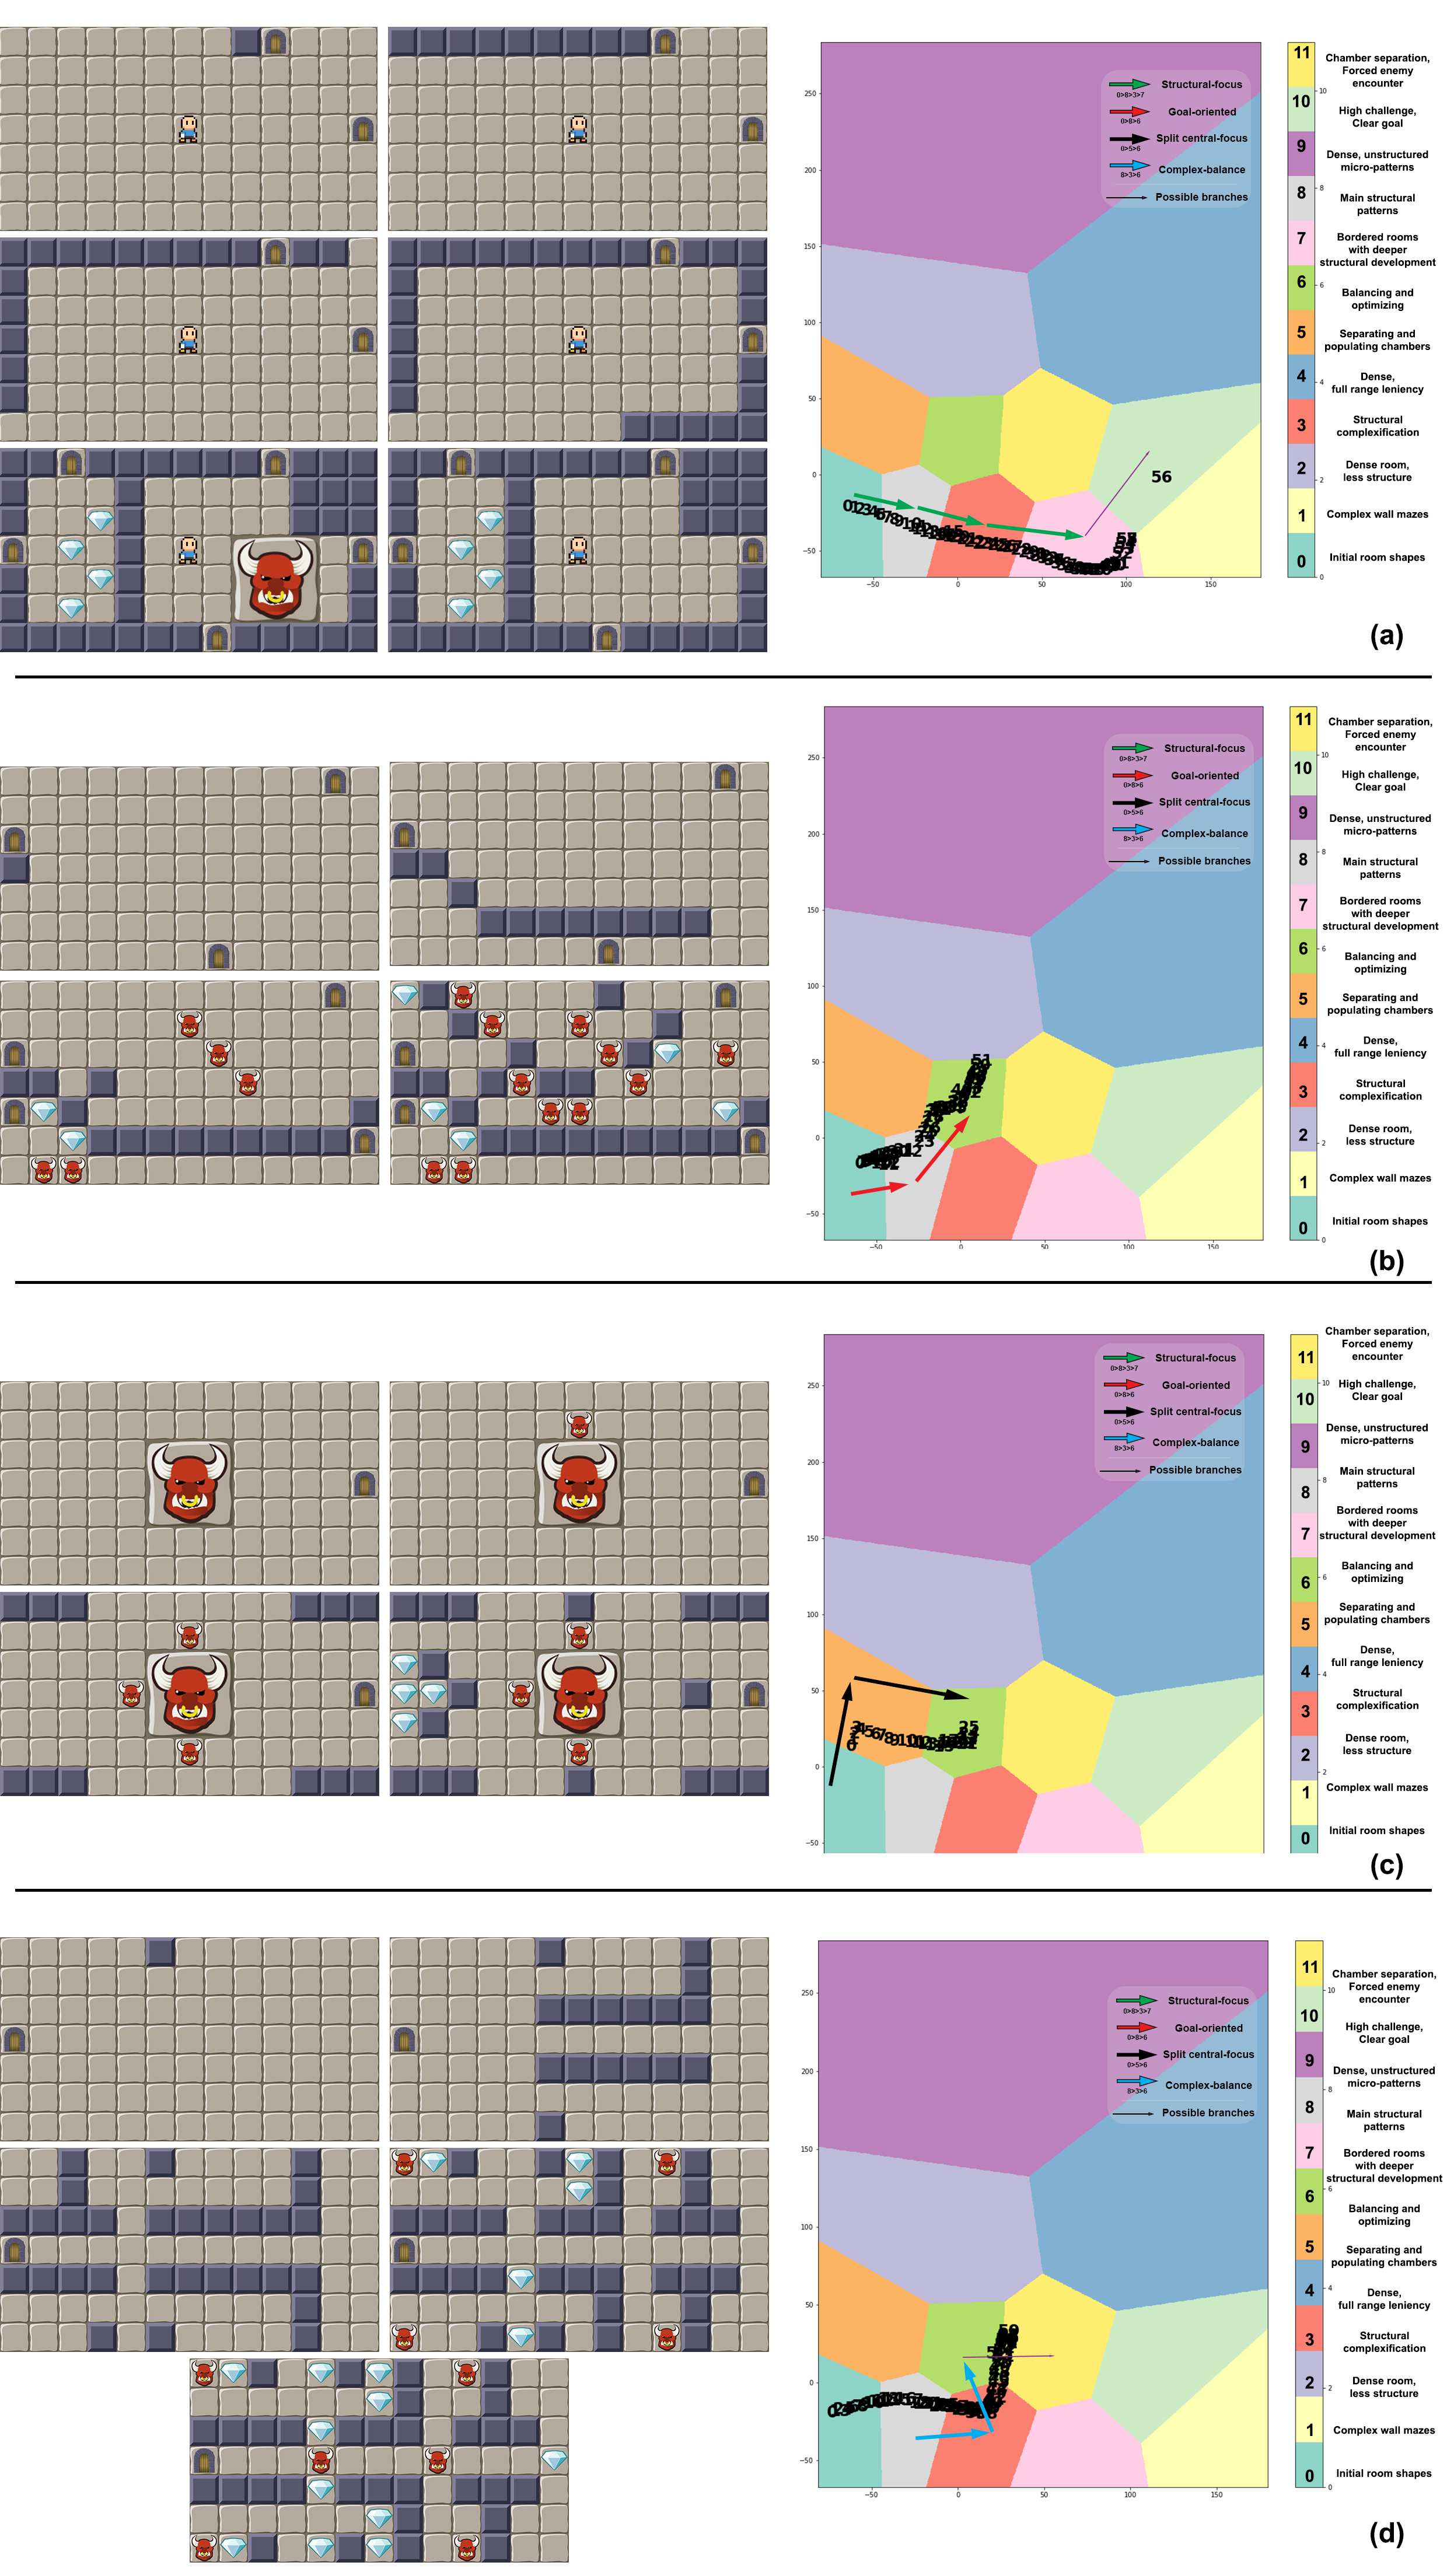
\includegraphics[width=0.7\textwidth]{figures/path-examples-2.png}}
% \caption{Examples of each of the archetypical paths from one of the frequent sequences used to create the clusters. To the left of each subfigure, we present each key step in the trajectory i.e. when the design entered a new cluster. (a) presents the \textsc{Structural focus} archetypical path where the focus is firstly on creating the structural design of the rooms; the design process jumps back and forth suddenly to cluster 10 (one of the possible branches) due to the designer adding a boss, and removing it immediately. (b) presents the \textsc{Goal-oriented} archetypical path where the design focus on a minimal structure complexity and mix between adding structural changes and enemies/treasures. (c) shows the \textsc{Split central-focus} archetypical path where intentionally, the designer creates a center obstacle with a boss and build around it. Finally, (d) presents the \textsc{Complex-balance} archetypical path; the design focuses on building complex uncommon structures first and then add some goal to it with enemies and treasures, taking advantage of the spaces.} \label{p6fig:archetypical-examples}
% \end{figure*}



% \begin{subfigure}[t]{0.33\textwidth}
%         \centering
%         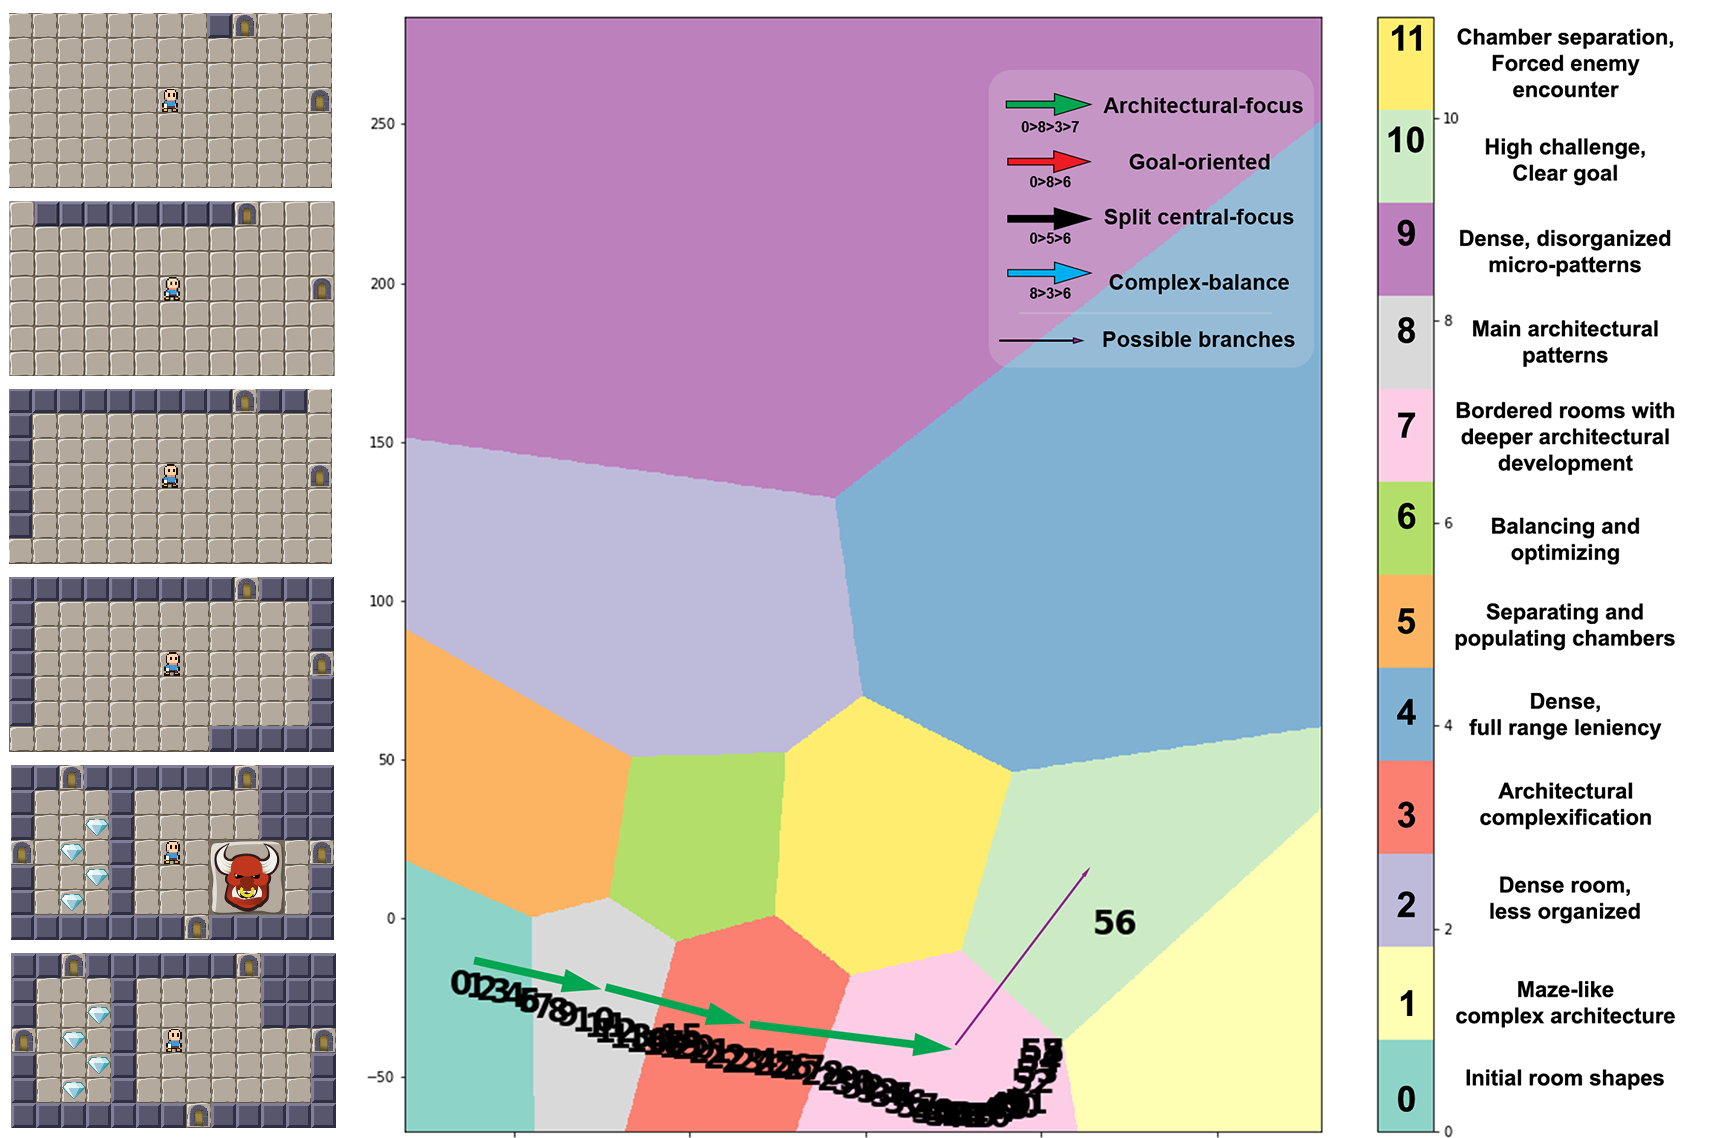
\includegraphics[width=0.95\textwidth]{figures/1.png}
%         \caption{Linearity-\#MesoPatterns}
%     \end{subfigure}%
%     \begin{subfigure}[t]{0.33\textwidth}
%         \centering
%         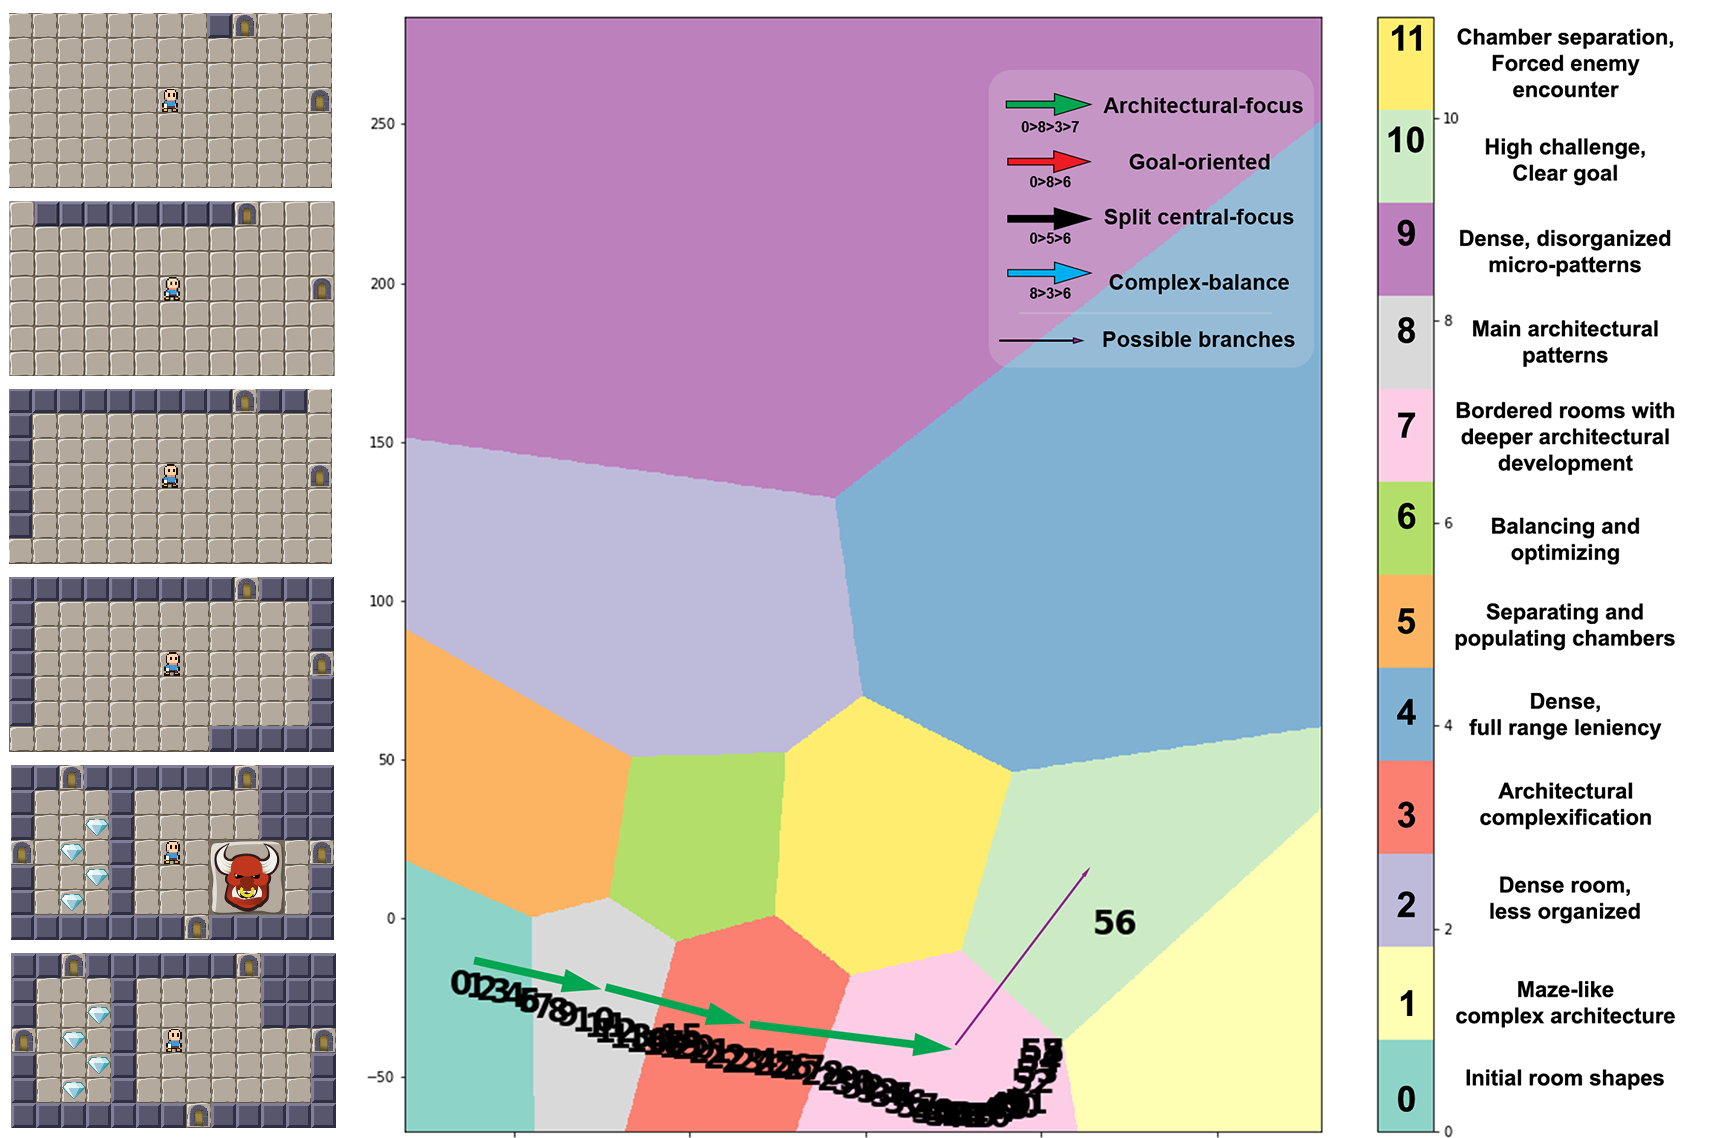
\includegraphics[width=0.95\textwidth]{figures/1.png}
%         \caption{Linearity-\#MesoPatterns}
%     \end{subfigure}%
%     \begin{subfigure}[t]{0.33\textwidth}
%         \centering
%         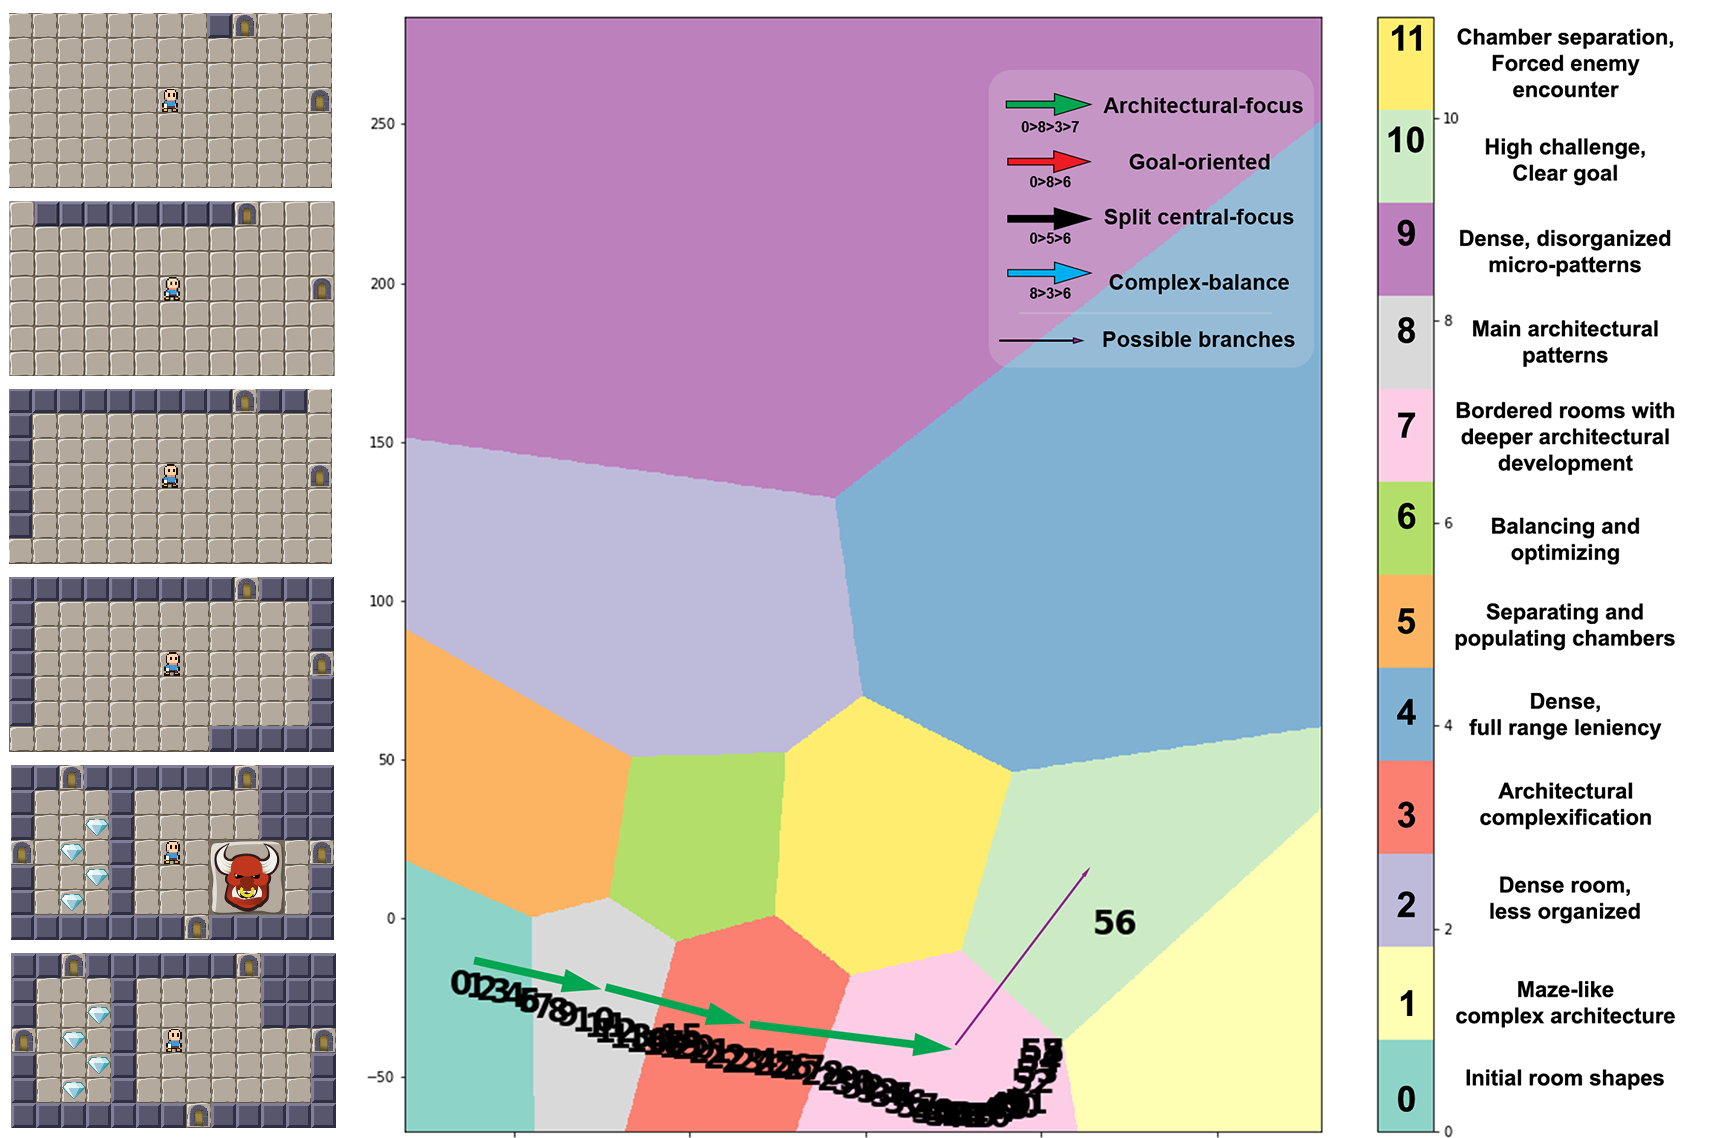
\includegraphics[width=0.95\textwidth]{figures/1.png}
%         \caption{Linearity-\#MesoPatterns}
%     \end{subfigure}%
%     \begin{subfigure}[t]{0.33\textwidth}
%         \centering
%         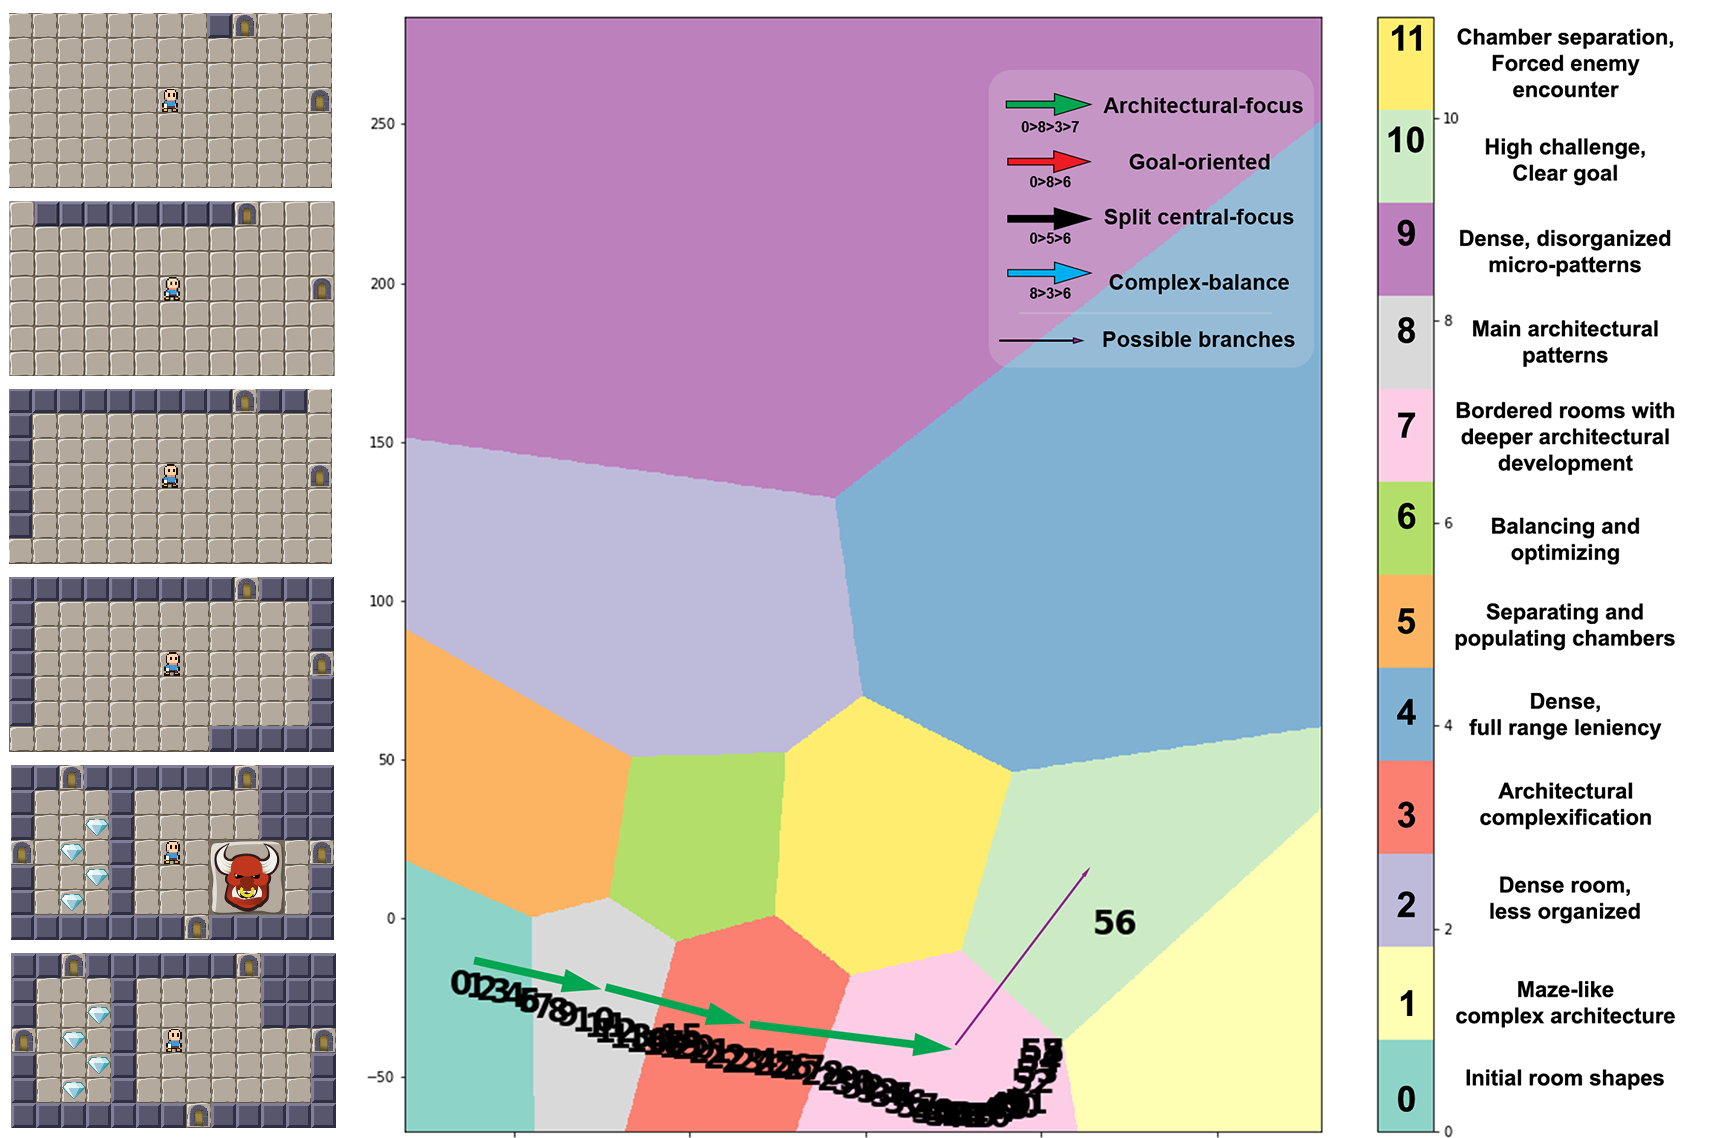
\includegraphics[width=0.95\textwidth]{figures/1.png}
%         \caption{Linearity-\#MesoPatterns}
%     \end{subfigure}%

%From the figure, it can be observed that most of the paths end or go through the "light green" and "light blue" clusters. Both relate to rooms that have a more clear structural pattern and more explicit mix between corridors and small chambers, thus, is understandable since the rooms in those clusters are or shaped as end rooms or structurally shaped to be “optimized” to a specific goal (E.g. dense bordered room, maze-like, more challenging, etc.). Further, most of the sequences end up


%Most of the rooms end there, 64 end in cluster 6 (light blue) and 52 end in cluster 11 (light green), so it makes sense that they are key steps in most of the subsequences. Further, most of the rooms start in cluster 0 (red) – 95 rooms – or in cluster 8 (purple) – 49 rooms, which make them key steps as well

%Most of the sequences with $95$ out of the $180$ starting in the red cluster, and $49$ out of the $180$ starting in the purple cluster. which correlates to the type of designs encountered in those clusters, mainly emptier rooms with initial sketches and shapes. 


%Info about the trajectories, 1) variation (length), 2) starting cluster, 3) end-point cluster.


% \begin{itemize}
%     \item[\textbf{DONE:}] Present 3 representative examples where we cluster each step of the design process. Perhaps I should create a room that would go through all the clusters?
%     \item[\textbf{DONE:}] Explain that we did this for all the 180 designs, and we collected the unique trajectories along the clusters, reducing the dimensionality of each step to each cluster.
%     \item[\textbf{DONE:}] Due to border designs (step that are in the border between 2 different clusters), we applied a threshold to reduce the noise those inputs could have when clustering the trajectories of the designer.
%     \item[\textbf{DONE:}] this data (the sequences) were then applied the GSP algorithm, a subsequence frequent pattern mining algorithm, to extract the frequent patterns in the sequences (including subsequences within the sequence).
%     \item This resulted in the following trajectories, which can also be observed in Figure X.
%     \item 
% \end{itemize}
